% Generated by benchmarks/src/utils/make_breakeven_figure.py -- do not hand-edit.
\definecolor{brk0}{HTML}{4285F4}
\definecolor{brk1}{HTML}{EA4335}
\definecolor{brk2}{HTML}{FBBC05}
\definecolor{brk3}{HTML}{EDA100}
\definecolor{brk4}{HTML}{E87BA4}
\definecolor{brk5}{HTML}{008300}
\definecolor{brk6}{HTML}{34A853}
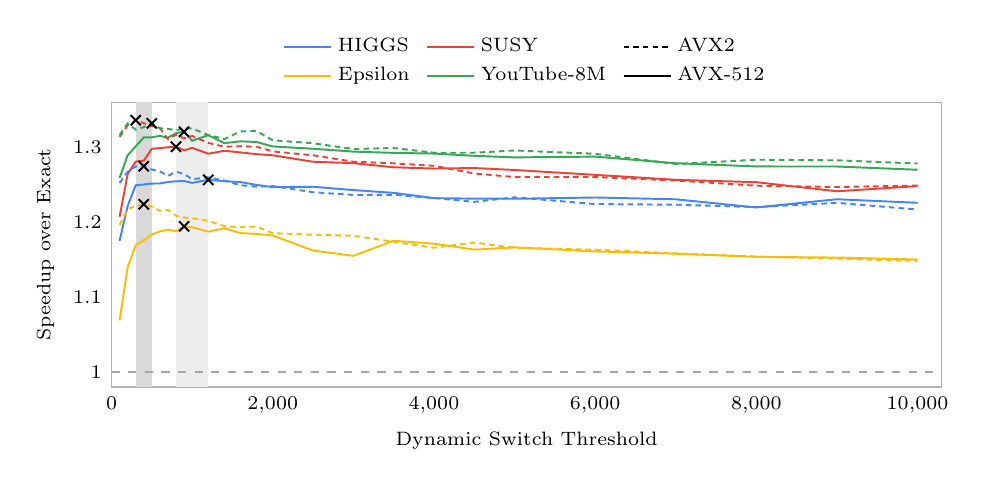
\begin{tikzpicture}
\begin{axis}[width=\linewidth, height=5.2cm, xmode=normal, xmin=0, xmax=10300,
  ymin=0.98, ymax=1.36, xtick={0,2000,4000,6000,8000,10000}, log ticks with fixed point,
  xlabel={Dynamic Switch Threshold},
  ylabel={Speedup over Exact}, tick label style={font=\scriptsize},
  label style={font=\scriptsize}, grid=none, axis line style={gray!60}, tick style={draw=none},
  every axis plot/.append style={line width=0.7pt, mark size=1.1pt},
  legend style={font=\scriptsize, draw=none, fill=none, at={(0.5,1.02)}, anchor=south, legend columns=3,
    /tikz/every even column/.append style={column sep=4pt}}, legend cell align=left,
  scaled x ticks=false, scaled y ticks=false, yticklabel style={/pgf/number format/fixed, /pgf/number format/precision=2}]
\fill[gray!14] (axis cs:800,0.98) rectangle (axis cs:1200,1.36);
\fill[gray!30] (axis cs:300,0.98) rectangle (axis cs:500,1.36);
\addplot[gray!70, dashed, line width=0.6pt, forget plot] coordinates {(0,1) (10300,1)};
\addplot[color=brk0, mark=none, solid, forget plot] coordinates {(100,1.1750) (200,1.2216) (300,1.2491) (400,1.2501) (500,1.2514) (600,1.2515) (700,1.2535) (800,1.2544) (900,1.2547) (1000,1.2523) (1200,1.2563) (1400,1.2546) (1600,1.2534) (1800,1.2496) (2000,1.2466) (2500,1.2471) (3000,1.2427) (3500,1.2390) (4000,1.2319) (4500,1.2313) (5000,1.2311) (6000,1.2328) (7000,1.2304) (8000,1.2195) (9000,1.2305) (10000,1.2257)};
\addplot[color=black, mark=x, mark size=2.6pt, only marks, forget plot] coordinates {(1200,1.2563)};
\addplot[color=brk1, mark=none, solid, forget plot] coordinates {(100,1.2072) (200,1.2639) (300,1.2808) (400,1.2819) (500,1.2978) (600,1.2987) (700,1.2998) (800,1.3006) (900,1.2956) (1000,1.2990) (1200,1.2912) (1400,1.2951) (1600,1.2929) (1800,1.2906) (2000,1.2891) (2500,1.2805) (3000,1.2786) (3500,1.2731) (4000,1.2714) (4500,1.2721) (5000,1.2695) (6000,1.2630) (7000,1.2564) (8000,1.2532) (9000,1.2411) (10000,1.2480)};
\addplot[color=black, mark=x, mark size=2.6pt, only marks, forget plot] coordinates {(800,1.3006)};
\addplot[color=brk2, mark=none, solid, forget plot] coordinates {(100,1.0690) (200,1.1397) (300,1.1691) (400,1.1758) (500,1.1836) (600,1.1875) (700,1.1900) (800,1.1877) (900,1.1943) (1000,1.1931) (1200,1.1873) (1400,1.1918) (1600,1.1853) (1800,1.1842) (2000,1.1821) (2500,1.1620) (3000,1.1550) (3500,1.1751) (4000,1.1712) (4500,1.1633) (5000,1.1663) (6000,1.1609) (7000,1.1578) (8000,1.1536) (9000,1.1527) (10000,1.1501)};
\addplot[color=black, mark=x, mark size=2.6pt, only marks, forget plot] coordinates {(900,1.1943)};
\addplot[color=brk6, mark=none, solid, forget plot] coordinates {(100,1.2589) (200,1.2890) (300,1.3010) (400,1.3129) (500,1.3131) (600,1.3150) (700,1.3125) (800,1.3187) (900,1.3205) (1000,1.3085) (1200,1.3160) (1400,1.3053) (1600,1.3077) (1800,1.3068) (2000,1.3009) (2500,1.2978) (3000,1.2940) (3500,1.2923) (4000,1.2914) (4500,1.2884) (5000,1.2863) (6000,1.2873) (7000,1.2785) (8000,1.2742) (9000,1.2741) (10000,1.2698)};
\addplot[color=black, mark=x, mark size=2.6pt, only marks, forget plot] coordinates {(900,1.3205)};
\addplot[color=brk0, mark=none, dash pattern=on 2pt off 1.5pt, forget plot] coordinates {(100,1.2521) (200,1.2671) (300,1.2742) (400,1.2745) (500,1.2701) (600,1.2676) (700,1.2616) (800,1.2672) (900,1.2641) (1000,1.2571) (1200,1.2598) (1400,1.2553) (1600,1.2491) (1800,1.2473) (2000,1.2481) (2500,1.2398) (3000,1.2362) (3500,1.2364) (4000,1.2321) (4500,1.2270) (5000,1.2330) (6000,1.2240) (7000,1.2232) (8000,1.2200) (9000,1.2256) (10000,1.2168)};
\addplot[color=black, mark=x, mark size=2.6pt, only marks, forget plot] coordinates {(400,1.2745)};
\addplot[color=brk1, mark=none, dash pattern=on 2pt off 1.5pt, forget plot] coordinates {(100,1.3136) (200,1.3289) (300,1.3359) (400,1.3319) (500,1.3281) (600,1.3254) (700,1.3105) (800,1.3166) (900,1.3117) (1000,1.3149) (1200,1.3056) (1400,1.3005) (1600,1.3012) (1800,1.3005) (2000,1.2943) (2500,1.2891) (3000,1.2805) (3500,1.2784) (4000,1.2750) (4500,1.2648) (5000,1.2601) (6000,1.2601) (7000,1.2555) (8000,1.2485) (9000,1.2468) (10000,1.2487)};
\addplot[color=black, mark=x, mark size=2.6pt, only marks, forget plot] coordinates {(300,1.3359)};
\addplot[color=brk2, mark=none, dash pattern=on 2pt off 1.5pt, forget plot] coordinates {(100,1.1960) (200,1.2175) (300,1.2212) (400,1.2237) (500,1.2208) (600,1.2148) (700,1.2163) (800,1.2086) (900,1.2059) (1000,1.2052) (1200,1.2017) (1400,1.1947) (1600,1.1931) (1800,1.1941) (2000,1.1852) (2500,1.1832) (3000,1.1818) (3500,1.1737) (4000,1.1658) (4500,1.1727) (5000,1.1657) (6000,1.1632) (7000,1.1583) (8000,1.1540) (9000,1.1513) (10000,1.1481)};
\addplot[color=black, mark=x, mark size=2.6pt, only marks, forget plot] coordinates {(400,1.2237)};
\addplot[color=brk6, mark=none, dash pattern=on 2pt off 1.5pt, forget plot] coordinates {(100,1.3162) (200,1.3314) (300,1.3233) (400,1.3267) (500,1.3317) (600,1.3250) (700,1.3244) (800,1.3223) (900,1.3251) (1000,1.3248) (1200,1.3161) (1400,1.3107) (1600,1.3210) (1800,1.3214) (2000,1.3091) (2500,1.3052) (3000,1.2974) (3500,1.2988) (4000,1.2925) (4500,1.2925) (5000,1.2955) (6000,1.2911) (7000,1.2774) (8000,1.2832) (9000,1.2824) (10000,1.2781)};
\addplot[color=black, mark=x, mark size=2.6pt, only marks, forget plot] coordinates {(500,1.3317)};
\addlegendimage{color=brk0, solid, line width=0.7pt, mark=none}
\addlegendentry{HIGGS}
\addlegendimage{color=brk1, solid, line width=0.7pt, mark=none}
\addlegendentry{SUSY}
\addlegendimage{color=black, dash pattern=on 2pt off 1.5pt, line width=0.7pt, mark=none}
\addlegendentry{AVX2}
\addlegendimage{color=brk2, solid, line width=0.7pt, mark=none}
\addlegendentry{Epsilon}
\addlegendimage{color=brk6, solid, line width=0.7pt, mark=none}
\addlegendentry{YouTube-8M}
\addlegendimage{color=black, solid, line width=0.7pt, mark=none}
\addlegendentry{AVX-512}
\end{axis}
\end{tikzpicture}
